\documentclass[12pt,a4paper]{report}
\usepackage{tgcommon}

\title{Relatório Técnico de Resultados Parciais}
\author{João Matheus Del Vecchio França Barbosa}
\date{2026}

\begin{document}
\tgtitlepage
  {João Matheus Del Vecchio França Barbosa}
  {Estimação Neural de Processos de Hawkes em Dados de Criptomoedas de Alta Frequência}
  {Relatório técnico de resultados parciais}
  {2026}

\pagenumbering{roman}
\begin{abstract}
Este relatório registra o estado executado do projeto que reproduz e estende
\citet{lee2023}. A contribuição planejada consiste em estimar os parâmetros de um
processo de Hawkes bidimensional por redes neurais em dados de alta frequência de
BTCUSDT e ETHUSDT. Foram construídos o repositório reproduzível, a ingestão dos dados
públicos da Binance, a transformação do top-of-book em eventos, o simulador de Hawkes,
o estimador de máxima verossimilhança, a LSTM de referência e o Transformer comparativo.
A janela principal, de 15 a 28 de janeiro de 2024, contém 1.826.904 eventos; a janela
de robustez, de 23 a 29 de outubro de 2023, contém 1.288.352 eventos. Testes
exploratórios confirmaram a integração dos componentes. A avaliação sintética final
usa 75.000 trajetórias de treino, 10.000 de validação e 15.000 de teste, todas com
1.000 eventos; LSTM e Transformer são agregados sobre cinco seeds e comparados ao MLE.
\end{abstract}

\tableofcontents
\clearpage
\pagenumbering{arabic}

\chapter{Objetivo e estado do trabalho}

O problema é estimar rapidamente
\[
  \theta=(\mu,\alpha_{\mathrm{self}},\alpha_{\mathrm{cross}},\beta)
\]
de um processo de Hawkes que representa mudanças para cima e para baixo no preço.
A máxima verossimilhança (MLE) é o referencial estatístico; a LSTM de \citet{lee2023}
é a reprodução; o Transformer é a extensão.

\begin{statusbox}
Este documento distingue os smoke tests de integração da avaliação final. As métricas
finais são geradas diretamente do resumo consolidado e incorporadas no capítulo de
comparação, evitando transcrição manual.
\end{statusbox}

Foram concluídos:
\begin{enumerate}
  \item a fonte e o mercado foram escolhidos com evidência de disponibilidade;
  \item 42 partições diárias foram processadas: 28 principais e 14 de robustez;
  \item o Hawkes 2D foi simulado pelo método de Ogata;
  \item o MLE foi implementado com restrições de estabilidade;
  \item LSTM e Transformer foram executados em cinco seeds no teste sintético congelado;
  \item o MLE foi ajustado separadamente nas 15.000 trajetórias desse teste;
  \item testes automatizados, lint e verificações dos artefatos foram executados.
\end{enumerate}

\chapter{Dados}

\section{Por que futuros USD-M}

O artigo-base usa NBBO de ações, isto é, a melhor oferta de compra e a melhor oferta
de venda. Para cripto, era necessário um equivalente. A Binance publica
\dataset{bookTicker} histórico para futuros USD-M, contendo melhor bid e ask, mas não
oferece o mesmo arquivo histórico oficial para spot. \dataset{aggTrades} existe nos
dois mercados, porém negócios realizados não permitem reconstruir sozinhos o
top-of-book. Logo, foram escolhidos futuros perpétuos USD-M \citep{binancePublicData}.

\section{Períodos}

\begin{table}[ht]
\centering
\caption{Janelas empíricas processadas.}
\begin{tabular}{llll}
\toprule
Uso & Período UTC & Símbolos & Produtos\\
\midrule
Principal & 15--28 jan. 2024 & BTCUSDT, ETHUSDT & bookTicker, aggTrades\\
Robustez & 23--29 out. 2023 & BTCUSDT, ETHUSDT & bookTicker, aggTrades\\
\bottomrule
\end{tabular}
\end{table}

O split principal foi congelado temporalmente:
\begin{itemize}
  \item 15--22 de janeiro: calibração e treino empírico;
  \item 23--25 de janeiro: validação;
  \item 26--28 de janeiro: teste fechado.
\end{itemize}
Janelas sobrepostas não podem cruzar essas fronteiras, pois isso copiaria eventos do
treino para validação ou teste.

\section{Transformação}

Para cada atualização:
\[
  m(t)=\frac{p_{\mathrm{bid}}(t)+p_{\mathrm{ask}}(t)}{2}.
\]
O último estado disponível em cada intervalo de 100 ms é mantido. Se o mid-price não
muda, não há evento. Se muda, registra-se tipo 1 para alta e tipo 2 para baixa, tempo
entre eventos e módulo do salto em ticks. BTCUSDT usa tick 0,1; ETHUSDT, 0,01.
O processamento é incremental, pois um único CSV diário pode ter 1,7 GB e quase
20 milhões de linhas.

\section{Cobertura principal}

\begin{table}[ht]
\centering
\caption{Resumo do dataset principal após filtragem.}
\begin{tabular}{lrr}
\toprule
Símbolo & Eventos & Segmentos de 1.000\\
\midrule
BTCUSDT & 887.803 & 880\\
ETHUSDT & 939.101 & 933\\
\midrule
Total & 1.826.904 & 1.813\\
\bottomrule
\end{tabular}
\end{table}

Todos os 56 arquivos esperados estavam disponíveis. Para o comprimento adotado no
protocolo final, o índice contém 1.813 janelas de 1.000 eventos. O menor dia ainda
contém 16.576 eventos em BTCUSDT e 20.828 em ETHUSDT.

\section{Robustez}

A janela de outubro produziu 652.773 eventos de BTCUSDT e 635.579 de ETHUSDT,
totalizando 1.288.352. Ela não foi usada para escolher arquitetura e deverá funcionar
como teste de mudança de regime temporal.

\chapter{Modelo de Hawkes}

\section{Intensidade}

Para tipos \(i,j\in\{1,2\}\),
\[
\lambda_i(t)=\mu+\sum_{j=1}^{2}\sum_{t_k^j<t}
  \alpha_{ij}\exp[-\beta(t-t_k^j)],
\]
com
\[
\boldsymbol{\alpha}=
\begin{bmatrix}
\alpha_{\mathrm{self}} & \alpha_{\mathrm{cross}}\\
\alpha_{\mathrm{cross}} & \alpha_{\mathrm{self}}
\end{bmatrix}.
\]
Um evento de alta aumenta imediatamente as intensidades; esse aumento decai à taxa
\(\beta\). A autoexcitação mede o efeito sobre o mesmo tipo, e a excitação cruzada
mede o efeito sobre o tipo oposto \citep{hawkes1971,bacry2013}.

\section{Estabilidade}

A razão de ramificação do modelo simétrico é
\[
  g=\frac{\alpha_{\mathrm{self}}+\alpha_{\mathrm{cross}}}{\beta}.
\]
Exige-se \(g<1\). Intuitivamente, cada evento precisa gerar, em média, menos de um
descendente direto; caso contrário, a cascata não morre. No código, a rede prevê uma
margem positiva \(d\) e define
\[
 \beta=\alpha_{\mathrm{self}}+\alpha_{\mathrm{cross}}+d,
 \qquad d=\softplus(z_4)>0.
\]
Isso garante a restrição por construção.

\chapter{Métodos implementados}

\section{Simulação}

O método de thinning de Ogata \citep{ogata1981} gera um tempo candidato a partir de uma
intensidade que limita a intensidade futura. O candidato é aceito com probabilidade
igual à razão entre intensidade real e limite. Após a aceitação, escolhe-se alta ou
baixa proporcionalmente às intensidades e atualiza-se o vetor de excitação.

\section{Máxima verossimilhança}

Para eventos \((t_k,c_k)\) observados até \(T\),
\[
 \ell(\theta)=\sum_k\log\lambda_{c_k}(t_k)
 -\sum_{i=1}^{2}\int_0^T\lambda_i(u)\,du.
\]
O código usa L-BFGS-B sobre parâmetros não restritos, transformados por softplus.
Foram empregados múltiplos pontos iniciais. Os seis ajustes de 1.000 eventos
reportados abaixo---dois símbolos e três splits---convergiram.

\begin{table}[ht]
\centering
\caption{Tempos dos ajustes MLE de 1.000 eventos.}
\begin{tabular}{llllr}
\toprule
Símbolo & Data & Split & Convergência & Tempo (s)\\
\midrule
BTCUSDT & 15 jan. & treino & sim & 2,02\\
BTCUSDT & 23 jan. & validação & sim & 1,33\\
BTCUSDT & 26 jan. & teste & sim & 1,93\\
ETHUSDT & 15 jan. & treino & sim & 2,77\\
ETHUSDT & 23 jan. & validação & sim & 1,68\\
ETHUSDT & 26 jan. & teste & sim & 1,74\\
\bottomrule
\end{tabular}
\end{table}

\section{LSTM}

A réplica possui duas camadas LSTM com 12 unidades e uma camada de saída com quatro
valores, conforme \citet{lee2023}. A entrada em cada passo é
\((\log(1+\Delta t),s)\), em que \(s=+1\) para alta e \(s=-1\) para baixa. A LSTM
\citep{hochreiter1997} comprime o histórico em um estado oculto, usado para prever
\(\theta\).

\section{Transformer}

O Transformer \citep{vaswani2017} projeta os dois atributos para dimensão interna,
adiciona codificação posicional senoidal, aplica autoatenção e agrega os estados por
média. A atenção permite comparar diretamente posições distantes, mas tem custo
quadrático no comprimento da sequência.

Na configuração final, cada vetor de dimensão 2 é projetado para \(d_{\mathrm{model}}=32\).
O encoding senoidal é somado antes de duas camadas encoder. Cada camada divide os
32 componentes em quatro cabeças de oito componentes, aplica autoatenção e uma rede
feed-forward \(32\rightarrow128\rightarrow32\). Após normalização, a média dos
estados ao longo dos 1.000 eventos produz um vetor de dimensão 32. A cabeça
softplus retorna \(\mu,\alpha_s,\alpha_c,d>0\) e constrói
\(\beta=\alpha_s+\alpha_c+d\); logo, \(g<1\) por construção.

\chapter{Resultados exploratórios}

\section{Experimento sintético reduzido}

Foram geradas 1.024 trajetórias de treino e 128 de teste, com 128 eventos e três épocas.

\begin{table}[ht]
\centering
\caption{Smoke test sintético; não é resultado final.}
\begin{tabular}{lrrr}
\toprule
Modelo & MSE de teste & Inferência (ms/sequência) & Saídas válidas\\
\midrule
LSTM & 0,0448 & 0,156 & 100\%\\
Transformer & 0,0328 & 0,793 & 100\%\\
\bottomrule
\end{tabular}
\end{table}

O Transformer teve MSE 26,7\% menor nessa execução, mas latência aproximadamente
5,1 vezes maior. Não se pode generalizar: o treino publicado por Lee usa 75.000
amostras, teste de 15.000 e geralmente mais de 300 épocas.

\section{Integração empírica}

Doze janelas de 1.000 eventos, rotuladas pelo MLE, foram usadas em um treino mínimo.
O MSE de treino foi 0,5038 para LSTM e 0,1800 para Transformer; 100\% das saídas
foram válidas. Como o valor é de treino e a amostra é minúscula, ele apenas prova que
dados reais percorrem toda a pipeline. Não mede generalização.

\section{Validação do protocolo final}

Um segundo smoke test validou o novo runner com shards persistidos, validação,
checkpoints, métricas por parâmetro e MLE sem inicialização-oráculo. Ele usou apenas
48/16/16 trajetórias e duas épocas com sequências de 1.000 eventos. Os MSEs foram
0,2286 (LSTM), 0,1176 (Transformer) e 0,0064 (MLE em duas trajetórias). Todas as
saídas neurais foram válidas. Esses valores verificam a execução do protocolo; o
pequeno orçamento impede qualquer conclusão comparativa.

\chapter{Limitações e riscos}

\begin{enumerate}
  \item Os dados originais de ações de Lee não estão públicos; a parte empírica é
  adaptação, não reprodução literal.
  \item O artigo diverge entre a menção textual ao comprimento da sequência e o tensor
  reportado; o protocolo final adota exclusivamente sequências de 1.000 eventos.
  \item Faixas exatas, seeds, batch size e vários hiperparâmetros não foram publicados.
  \item A excitação cruzada do MLE ficou próxima de zero em 89\% das 1.063 janelas de
  calibração, e nenhuma janela cai dentro das faixas usadas no treino sintético
  (Capítulo~\ref{cap:atualizacao}); a avaliação empírica exige recalibrar o prior.
  \item O mercado 24/7 é não estacionário; splits e janela de robustez mitigam, mas
  não eliminam esse risco.
  \item O teste empírico fechado ainda requer avaliação com checkpoints congelados; ele
  é distinto do teste sintético final reportado neste documento.
\end{enumerate}

\chapter{Comparação final: LSTM, Transformer e MLE}

\section*{Resultados da execução final otimizada}

O protocolo final usa exclusivamente trajetórias de 1.000 eventos, com
75.000 amostras de treino, 10.000 de validação e 15.000 de teste.
As redes são resumidas sobre cinco seeds independentes; o MLE é ajustado
separadamente em cada trajetória do mesmo conjunto de teste.
Os intervalos das redes usam a distribuição $t$ de Student entre seeds.

\begin{table}[htbp]
\centering
\caption{Métricas agregadas no teste sintético congelado (15.000 trajetórias de 1.000 eventos).}
\label{tab:final-agregado}
\small
\begin{tabular}{lrrrrr}
\toprule
Estimador & MSE macro & IC 95\% & MAE macro & MSE de $g$ & Validade\\
\midrule
LSTM & 0,019618 & [0,013252; 0,025984] & 0,094276 & 0,001825 & 100,00\%\\
Transformer & 0,023700 & [0,019128; 0,028272] & 0,105642 & 0,002138 & 100,00\%\\
MLE & 0,506193 & -- & 0,111852 & 0,002344 & 100,00\%\\
\bottomrule
\end{tabular}
\end{table}

\begin{table}[htbp]
\centering
\caption{MSE de teste por parâmetro (redes: média de cinco seeds).}
\label{tab:final-parametros}
\begin{tabular}{lrrrr}
\toprule
Estimador & $\mu$ & $\alpha_{\mathrm{self}}$ & $\alpha_{\mathrm{cross}}$ & $\beta$\\
\midrule
LSTM & 0,002296 & 0,016222 & 0,016566 & 0,043386\\
Transformer & 0,002366 & 0,020905 & 0,021196 & 0,050332\\
MLE & 0,010108 & 0,006146 & 0,006214 & 2,002303\\
\bottomrule
\end{tabular}
\end{table}

\begin{table}[htbp]
\centering
\caption{MSE macro por regime da razão de ramificação $g$.}
\label{tab:final-regimes}
\begin{tabular}{lrrr}
\toprule
Estimador & $g$ baixo & $g$ intermediário & $g$ quase crítico\\
\midrule
LSTM & 0,019941 & 0,015614 & 0,023297\\
Transformer & 0,022228 & 0,018964 & 0,029908\\
MLE & 1,480568 & 0,016795 & 0,021214\\
\bottomrule
\end{tabular}
\end{table}

Entre as redes, a LSTM obteve MSE macro médio 17,2\% menor que o Transformer.
Com 5 e 5 seeds, porém, a diferença não é estatisticamente significativa (teste de Welch, $p=0,19$), e os intervalos de confiança se sobrepõem; os dados não permitem ordenar as redes.
No MLE, o parâmetro $\beta$ respondeu por 98,9\% da soma dos erros quadráticos,
e o MSE macro no regime de $g$ baixo foi 88,15 vezes o do regime intermediário:
com excitação fraca, $\beta$ é pouco identificado e algumas trajetórias
produzem estimativas extremas. Fora desse regime, o MLE é competitivo:
no regime intermediário, seu MSE macro foi 0,0168 (LSTM: 0,0156; Transformer: 0,0190) e, no
quase crítico, 0,0212 (LSTM: 0,0233; Transformer: 0,0299).
O MLE obteve o menor MSE entre os três estimadores em $\alpha_{\mathrm{self}}$ e $\alpha_{\mathrm{cross}}$.
Portanto, o MSE macro agregado não ordena os estimadores de forma robusta,
e convergência numérica não implica boa recuperação paramétrica.

\begin{figure}[htbp]
\centering
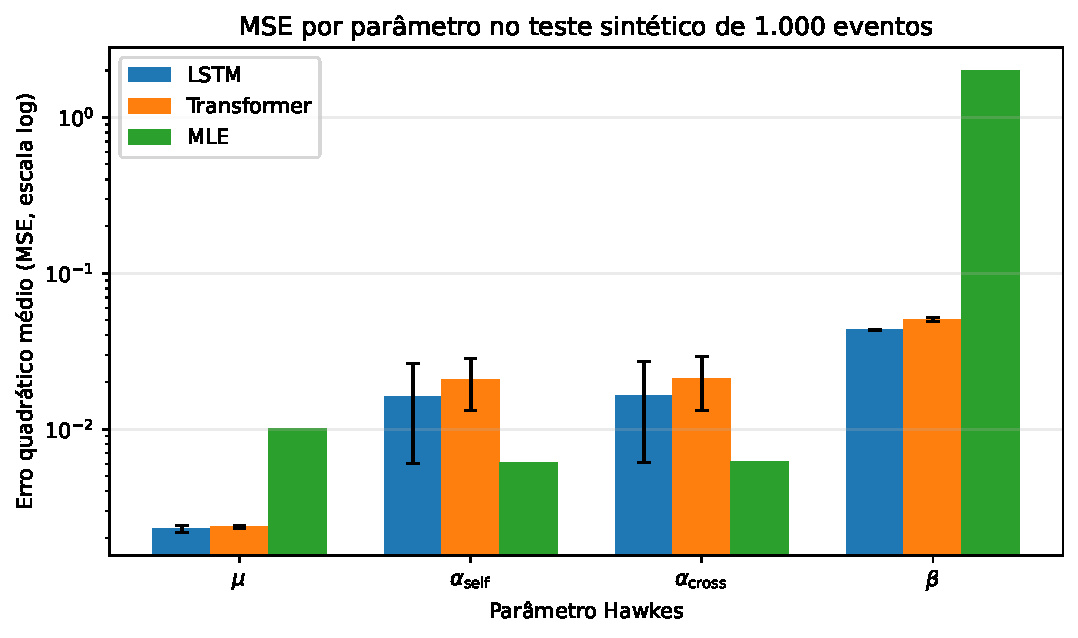
\includegraphics[width=0.88\linewidth]{../build/figures/parameter_mse.pdf}
\caption{MSE de teste por parâmetro no protocolo de 1.000 eventos.
As barras de erro das redes representam um desvio-padrão entre seeds.}
\end{figure}

\begin{figure}[htbp]
\centering
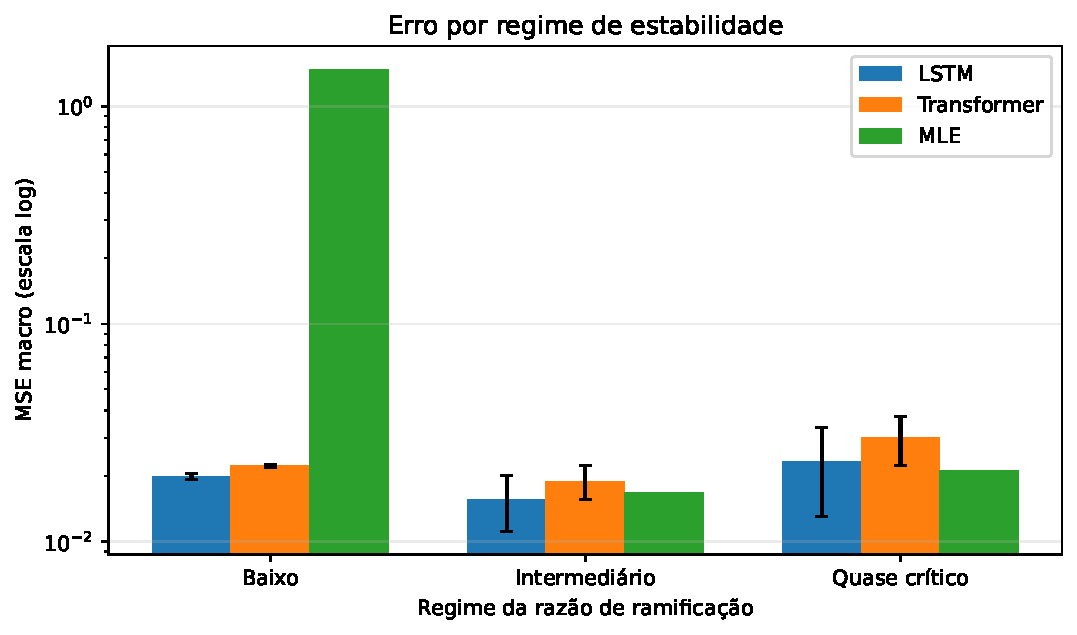
\includegraphics[width=0.88\linewidth]{../build/figures/branching_regime_mse.pdf}
\caption{MSE macro por regime da razão de ramificação. As barras de erro
das redes representam um desvio-padrão entre seeds.}
\end{figure}

\begin{figure}[htbp]
\centering
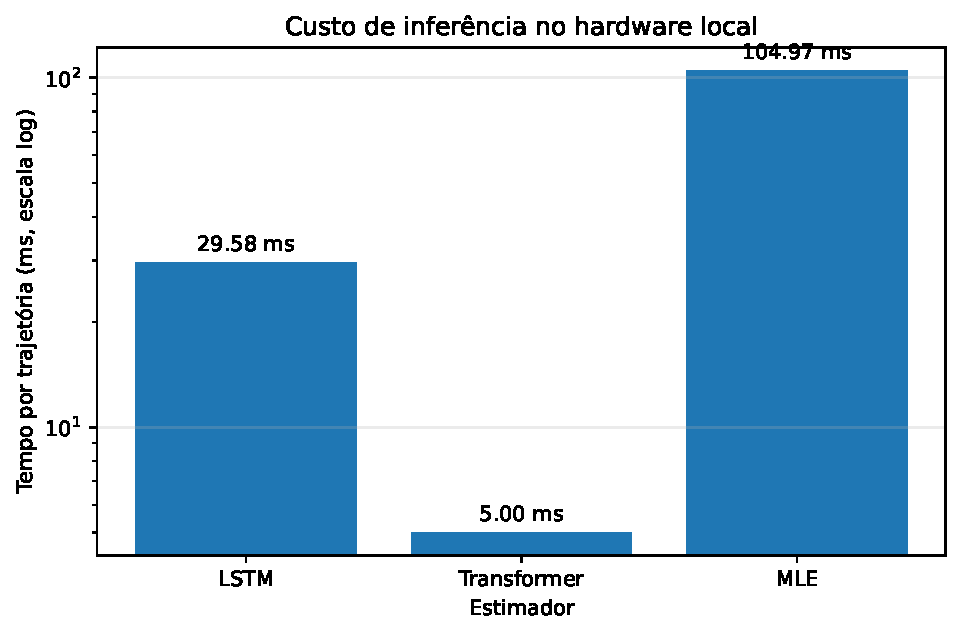
\includegraphics[width=0.80\linewidth]{../build/figures/inference_cost.pdf}
\caption{Custo por trajetória registrado durante a execução final, em escala
logarítmica. Para o MLE, tempo de parede com quatro processos que concorriam
com o treino na GPU; para as redes, latência mediana em batch unitário no
MPS. Um benchmark controlado posterior mediu cerca de 10~ms por trajetória
para o MLE em um único núcleo e deve ser preferido a esta figura.}
\end{figure}

O MLE convergiu em 100,00\% das trajetórias
e usou mediana de 14,00 iterações.
Todas as comparações usam o mesmo conjunto de teste congelado.


\chapter{Atualização de 30/10/2026: análise complementar}
\label{cap:atualizacao}

Este capítulo acrescenta análises feitas depois da execução final, sem retreino e sem
abrir o teste empírico: o experimento E2 no ponto fixo de \citet{lee2023}, métricas
robustas e testes pareados no teste sintético, o diagnóstico do MLE e a calibração em
janelas reais. Um benchmark controlado também mostrou que o MLE custa cerca de 10~ms
por trajetória em um núcleo, e não 105~ms, valor registrado enquanto o treino ocupava
a GPU.

\section{Ponto fixo do artigo (E2)}

\begin{table}[htbp]
\centering
\caption{Distribuição amostral no ponto fixo de \citet{lee2023} ($\mu=0{,}3$, $\alpha_{\mathrm{self}}=0{,}4$, $\alpha_{\mathrm{cross}}=0{,}7$, $\beta=1{,}5$): média e desvio-padrão em 2.000 trajetórias de 1.000 eventos. As linhas de Lee usam 100.000 trajetórias de 2.000 passos.}
\label{tab:e2-ponto-fixo}
\scriptsize
\begin{tabular}{lrrrrrrrr}
\toprule
 & \multicolumn{2}{c}{$\mu$} & \multicolumn{2}{c}{$\alpha_{\mathrm{self}}$} & \multicolumn{2}{c}{$\alpha_{\mathrm{cross}}$} & \multicolumn{2}{c}{$\beta$}\\
Estimador & Média & DP & Média & DP & Média & DP & Média & DP\\
\midrule
LSTM (ensemble de 5 seeds) & 0,3044 & 0,0365 & 0,4950 & 0,0536 & 0,6245 & 0,0608 & 1,5318 & 0,1436\\
Transformer (ensemble de 5 seeds) & 0,2957 & 0,0388 & 0,5280 & 0,0561 & 0,6055 & 0,0620 & 1,5308 & 0,1541\\
MLE heurístico (5 inícios) & 0,3065 & 0,0370 & 0,3956 & 0,0728 & 0,7075 & 0,0859 & 1,5156 & 0,1642\\
MLE oráculo (início no verdadeiro) & 0,3065 & 0,0370 & 0,3956 & 0,0728 & 0,7075 & 0,0859 & 1,5156 & 0,1642\\
Lee (2023) rede & 0,3151 & 0,0358 & 0,4429 & 0,0661 & 0,5733 & 0,0697 & 1,5736 & 0,1364\\
Lee (2023) MLE & 0,3036 & 0,0314 & 0,3988 & 0,0500 & 0,7024 & 0,0608 & 1,5078 & 0,1145\\
\bottomrule
\end{tabular}
\end{table}


\section{Análise complementar dos resultados sintéticos}
\label{sec:posthoc}

As previsões por trajetória foram recalculadas a partir dos checkpoints
congelados (diferença relativa máxima de $10^{-8}$ em relação ao MSE reportado),
sem retreino e sem alterar o protocolo. Como os parâmetros têm escalas
diferentes, cada erro quadrático é dividido pela variância do parâmetro no
conjunto de treino; o resultado complementar é o $R^2$ em relação ao
estimador trivial que sempre prevê a média a priori.

\begin{table}[htbp]
\centering
\caption{$R^2$ por parâmetro em relação à média a priori, erro absoluto
mediano macro e MSE da razão de ramificação no teste sintético.}
\label{tab:posthoc-r2}
\small
\begin{tabular}{lrrrrrr}
\toprule
Estimador & $\mu$ & $\alpha_{\mathrm{self}}$ & $\alpha_{\mathrm{cross}}$ & $\beta$ & EA mediano & MSE de $g$\\
\midrule
Média a priori & $-$0,01 & 0,00 & $-$0,01 & 0,01 & 0,1908 & 0,0670\\
MLE & 0,24 & 0,90 & 0,90 & $-$15,64 & 0,0674 & 0,0023\\
LSTM (ensemble) & 0,84 & 0,82 & 0,81 & 0,65 & 0,0680 & 0,0017\\
Transformer (ensemble) & 0,84 & 0,74 & 0,73 & 0,61 & 0,0765 & 0,0019\\
\bottomrule
\end{tabular}
\end{table}

\begin{table}[htbp]
\centering
\caption{Comparação pareada por trajetória (erro quadrático padronizado médio
nos quatro parâmetros). Colunas: perda mediana de A e de B, fração de
trajetórias em que A erra menos e IC 95\% \emph{bootstrap} da diferença média
A$-$B (negativo favorece A).}
\label{tab:posthoc-pareado}
\footnotesize
\begin{tabular}{llrrrr}
\toprule
A $\times$ B & Regime & Med.\ A & Med.\ B & A melhor & IC 95\% (A$-$B)\\
\midrule
LSTM $\times$ Transformer & todos & 0,151 & 0,187 & 70,2\% & [$-$0,051; $-$0,047]\\
LSTM $\times$ Transformer & $g$ baixo & 0,112 & 0,131 & 61,1\% & [$-$0,021; $-$0,016]\\
LSTM $\times$ Transformer & $g$ intermediário & 0,127 & 0,164 & 72,8\% & [$-$0,045; $-$0,041]\\
LSTM $\times$ Transformer & $g$ quase crítico & 0,237 & 0,304 & 76,7\% & [$-$0,089; $-$0,081]\\
\midrule
LSTM $\times$ MLE & todos & 0,151 & 0,149 & 48,8\% & [$-$9,394; $-$0,809]\\
LSTM $\times$ MLE & $g$ baixo & 0,112 & 0,199 & 63,5\% & [$-$26,977; $-$2,225]\\
LSTM $\times$ MLE & $g$ intermediário & 0,127 & 0,100 & 40,1\% & [$-$0,040; $-$0,009]\\
LSTM $\times$ MLE & $g$ quase crítico & 0,237 & 0,183 & 42,7\% & [$-$0,467; $-$0,277]\\
\midrule
Transformer $\times$ MLE & todos & 0,187 & 0,149 & 43,5\% & [$-$9,376; $-$0,782]\\
Transformer $\times$ MLE & $g$ baixo & 0,131 & 0,199 & 59,4\% & [$-$27,686; $-$2,207]\\
Transformer $\times$ MLE & $g$ intermediário & 0,164 & 0,100 & 34,2\% & [0,002; 0,035]\\
Transformer $\times$ MLE & $g$ quase crítico & 0,304 & 0,183 & 36,7\% & [$-$0,374; $-$0,195]\\
\bottomrule
\end{tabular}
\end{table}

Primeiro, a vantagem das redes sobre
o MLE no MSE agregado vem de poucas trajetórias: 94,4\% da soma
dos erros quadráticos de $\beta$ do MLE se concentra em 1\% das trajetórias,
quase todas no regime de $g$ baixo. Em todas as 300 piores, a log-verossimilhança
no estimador supera a do parâmetro verdadeiro (ganho mediano de 2,80), e reajustar
100 delas com 20 inícios praticamente não altera o resultado. Não é
falha numérica: com excitação fraca, $\beta$ é pouco identificado em 1.000
eventos. Segundo, na trajetória típica o MLE é tão bom quanto as redes ou
melhor: a perda mediana é praticamente igual à da LSTM no agregado e menor nos
regimes intermediário e quase crítico. Terceiro, na comparação pareada o
ensemble LSTM supera o ensemble Transformer em todos os regimes; entre seeds
isoladas, contudo, a diferença não é significativa (Welch, $p=0,19$;
Mann--Whitney, $p=0,056$), porque a LSTM
apresentou dois níveis de convergência entre seeds.

\begin{figure}[htbp]
\centering
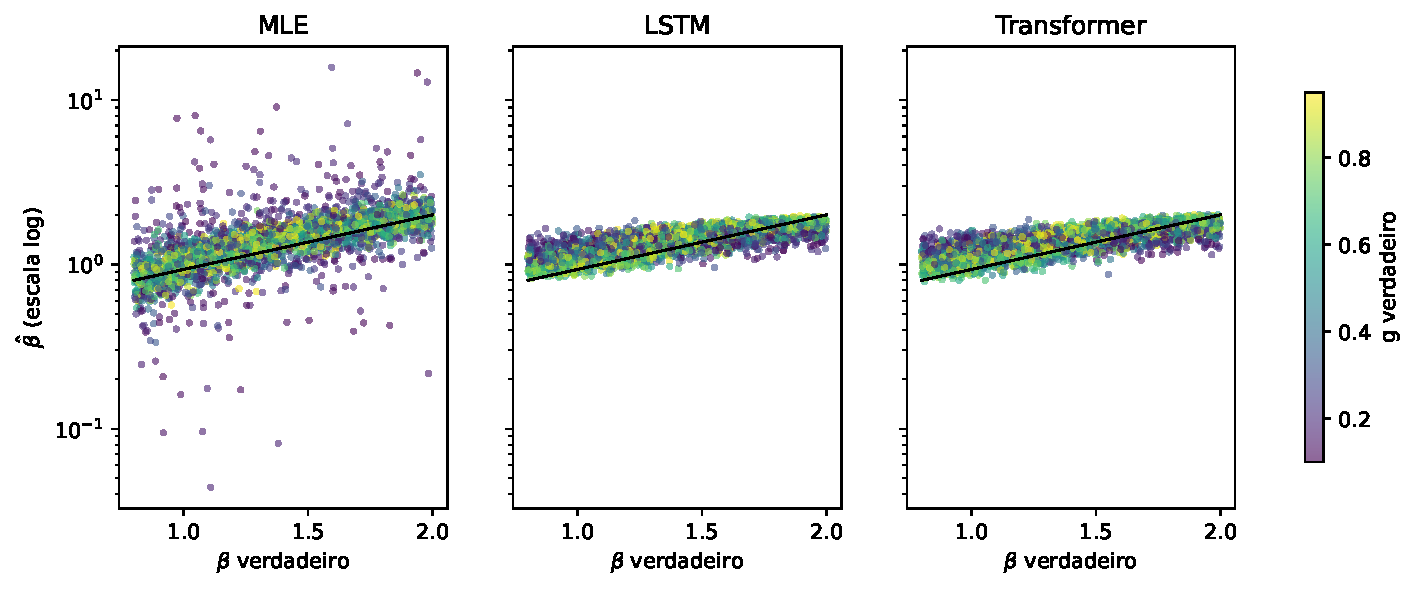
\includegraphics[width=0.95\linewidth]{../build/figures/posthoc_beta_verdadeiro_vs_estimado.pdf}
\caption{$\beta$ verdadeiro versus estimado (3.000 trajetórias de teste,
escala logarítmica). As redes encolhem as estimativas para o centro do
prior; o MLE é não viesado na maior parte do domínio, mas produz valores
extremos quando $g$ é baixo.}
\label{fig:posthoc-beta}
\end{figure}

\section{Calibração empírica e suporte do prior sintético}
\label{sec:calibracao}

O MLE foi ajustado nas 1063 janelas de 1.000 eventos do
bloco \texttt{calibration\_train} (15 a 22 de janeiro de 2024), único bloco
autorizado para calibração. A mediana de $\beta$ foi 2,71 (intervalo
interquartil 2,21--3,14), acima do limite de 2,0 usado no treino, e
$\alpha_{\mathrm{cross}}$ ficou abaixo de $10^{-3}$ em 89,4\% das janelas.
Apenas 15,4\% das janelas têm $\beta$ dentro do
prior, 0,4\% têm a fração autoexcitada
dentro de $[0{,}2;\,0{,}8]$ e 0,0\% satisfazem
todas as faixas ao mesmo tempo. Como um estimador treinado com perda
quadrática aproxima a média a posteriori sob o prior de treino, as redes
atuais não podem produzir estimativas nessa região; a avaliação empírica
exige recalibrar o prior ou treinar com rótulos MLE em janelas reais.

\begin{figure}[htbp]
\centering
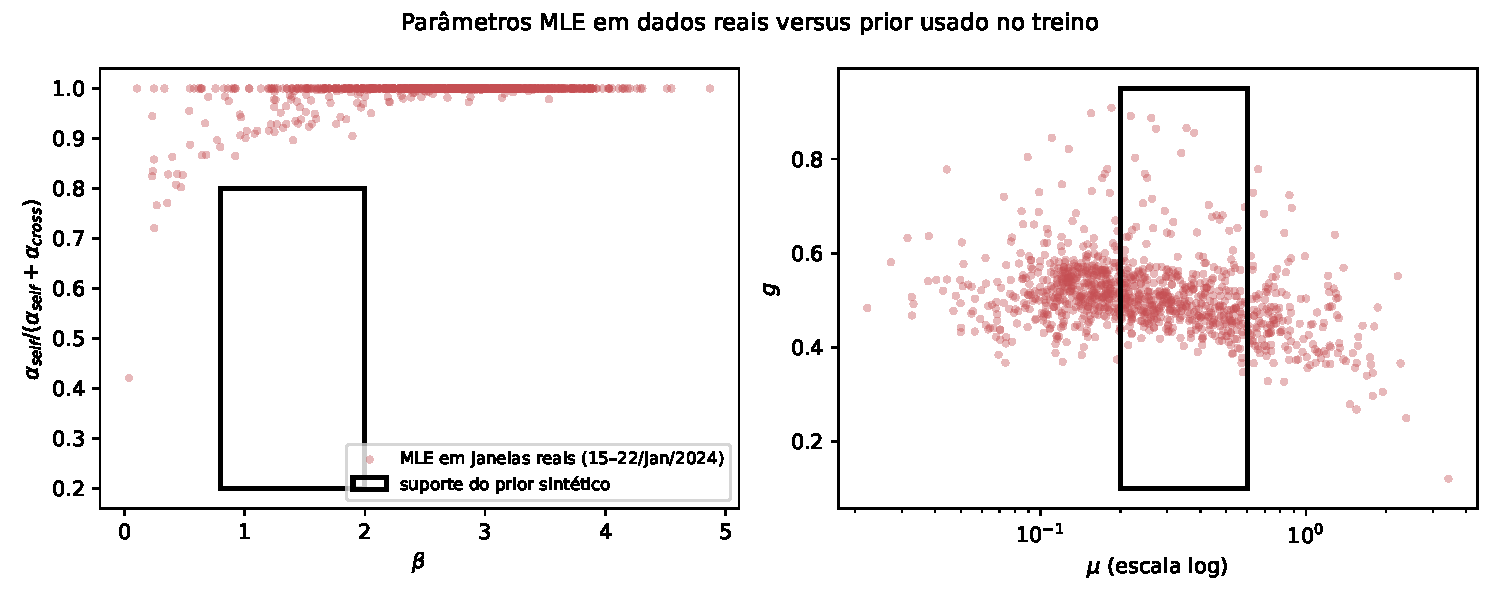
\includegraphics[width=0.95\linewidth]{../build/figures/posthoc_calibracao_vs_prior.pdf}
\caption{Estimativas MLE nas janelas reais de calibração (pontos) e suporte
do prior usado para gerar os dados de treino (retângulos).}
\label{fig:calibracao-prior}
\end{figure}


\chapter{Próximas etapas}

\begin{enumerate}
  \item treinar com rótulos MLE em janelas reais ou recalibrar o prior pelas 1.063
  janelas de calibração e retreinar;
  \item abrir o teste empírico após congelar a escolha e avaliar outubro sem retreinar;
  \item calcular volatilidade Hawkes e realized volatility \citep{andersen2003};
  \item ampliar a análise de sensibilidade sem ajustar decisões no teste sintético.
\end{enumerate}

\appendix
\chapter{Comandos de reprodução}

\begin{lstlisting}[language=bash]
uv sync --python 3.13 --extra dev
uv run python scripts/build_primary_dataset.py --workers 4
uv run python scripts/index_event_windows.py
uv run python scripts/run_empirical_mle.py --max-per-split 1
uv run python scripts/run_model_comparison.py \
  --train-size 1024 --test-size 128 --sequence-length 128 --epochs 3
uv run ruff check .
uv run mypy src/hawkes_crypto
uv run pytest
\end{lstlisting}

\bibliographystyle{plainnat}
\bibliography{references}
\end{document}

